 We have shown the gender bias issue in the coreference systems. In this section, we are going to propose methods to reduce the gender bias.
% What we do here is that we have the access to the training dataset and we will try to fix the problem by just adding some redundant information based on the original training dataset. 
The first method is  to add some redundant information based on the original training dataset. Without changing any training procedure or losing any useful information, we can show that this algorithm can help to reduce the gender bias in the coreference systems.
As the word embeddings also shows implicit gender bias issue~\cite{BCWS16}, the coreference systems using the word embeddings will also inherit such problem.  Besides the data augmentation method, we also  incorporate the debiased word embeddings for the calibration.

% \subsection{Strategies for Calibration}




% %Because the new corpus neutralizes the effect of gender biases by having b
% %we improve the huge difference between female and male. For instance, in previous dataset, for one specific job title such as ``leader'', every time it occurs in a cluster related to male. But in this new dataset, we have at least several times for female to relate to ``leader''.  Based on the adversarial training dataset, we retrain a new model. In this new model, all the information in the previous model still exists and the new information we added is just something we can simply achieve from the original dataset which means  our new model can at least maintain the previous performance and do not requiring a new strategy or a new loss function.

% To attest the efficiency of our algorithm, we conduct experiments measuring the performance of coreference resolution systems on the original and the Winograd datasets we collected. As the Stanford Deterministic system is a rule-based system, we cannot  retrain its model. We present the result for the calibration in the other two systems and show that the proposed approach reduces gender bias while maintaining strong performance when evaluated on the original data. 


\subsection{Results}

We show the performance of the three coreference resolution systems before and after retraining using our calibration in Table~\ref{tab:cluster_gender_ratio}.
Before adopting our calibration method, the UW system shows $21\%$ difference on the type1 wino dataset.
After the ART method, the difference shrinks to $5.95$. Also, with the DRT method, we can  reduce the gap to $7.94\%$ which means both method can help to mitigate the gender bias issue in the system. However the DART method, which makes the difference to $1.1\%$, shows the best performance in reducing the gender bias.

%  We can see that, after we trained on the union dataset, the evaluation on the original development split for the Berkeley coref system changes to $61.84\%$ from $61.71\%$, rising $0.13\%$, which demonstrates that our algorithm can keep the original performance. Also, the evaluation on the development split of the gender-reversed dataset changes from  $60.13\%$ to $61.90\%$ representing a $1.73\%$ improvement. 
 
% Results using the UW coref system also show the same trend. We keep the original performance at $67.47\%$ on the original development set and raise the performance on the gender-reversed development set from $66.44\%$ to $67.41\%$. All the results show that retraining on the dataset union does not hurt performance but in fact the model can gain more information to get better performance in the modified dataset. 
% After adopting ART, the distance between the performance in the original and gender-reversed dataset does not change much, which means the model is less sensitive to different genders. For the Berkeley coref system, the difference shrinks from $1.61\%$ to $-0.06\%$. The negative value here means the performance is better in the gender-reversed development dataset. And for the UW coref system, this difference changes from $1.26\%$ to $0.06\%$.

% \begin{table}[t]
% \centering
%     \begin{tabular}{|l|c|c|}
 
%         \hline
%          \bf System & \bf  Original Perf.& \bf Reversed  Perf.\\
%           \hline
%           \multicolumn{3}{|c|}{Development Set} \\
%           \hline
%         Berkeley &  61.84  &  61.90 \\
%         \hline
%         UW e2e  &   67.47  & 67.41   \\
%         \hline
%         \multicolumn{3}{|c|}{Test Set} \\
%           \hline
%         Berkeley &  60.96  & 60.95  \\
%         \hline
%         UW e2e  &   67.0  &  66.93   \\
%         \hline  
%     \end{tabular}
%     \caption{Performance after adopting our ART algorithm. We can see here the performance on the reversed evaluation dataset no longer drops acutely, which means we can effectively help to reduce the gender bias in these two coreference systems.
%     }
%     \label{tab:calibration}
% \end{table}


% In the prediction results, we find our algorithm can help to reduce the big difference on the cluster-level gender ratio. 
% Using the Berkeley coref system as an example, we show the gender ratio results on different datasets in Table~\ref{tab:cluster_gender_ratio}. After adopting our algorithm, the gender ratio on the original development dataset reduces from $79.1\%$ to $75.9\%$ which means in the predictions, more females are predicted and they can refer to more nouns or even more job titles. When predicting on the gender-reversed dataset, as female is now the primary gender, the gender ratio should be biased toward female. After using ART, the gender ratio is more biased toward female which means our model learns more information of females than the original model. 

% \begin{table*}[th]
% \centering
%     \begin{tabular}{|l|c|c|c|c|c|}
 
%         \hline
%         \bf System &
%          \bf Dataset & \bf  \#Male & \bf \#Female & \bf Male\% & \bf Female\%\\
%           \hline
%           -- & Gold & 441 & 111 & 79.9 & 20.1 \\
%           \hline
%           \multicolumn{6}{|c|}{Without ART} \\
%           \hline
%           \multirow{2}{*}{Berkeley} &
%         Original &  432  &  114 & 79.1 & 20.9 \\
%         \cline{2-6}
%         & Reversed  &   115  & 329 & 25.9 & 74.1  \\
%         \hline 
%         \multirow{2}{*}{UW e2e} 
%         & Original & 392 & 101 & 79.5 & 20.5 \\
%         \cline{2-6}
%         & Reversed & 120 & 407 & 22.8 & 77.2 \\
%         \hline
%         \multicolumn{6}{|c|}{With ART} \\
%         \hline
%         \multirow{2}{*}{Berkeley} &
%         Original &  444  & 141 & 75.9 & 24.1 \\
%         \cline{2-6}
%       &  Reversed  &  130   & 483 & 21.2 & 78.8  \\
%         \hline
%         \multirow{2}{*}{UW e2e} 
%         & Original & 394 & 121 & 76.5 & 23.5 \\
%         \cline{2-6}
%         & Reversed & 118 & 460 & 20.4 & 79.6 \\
%         \hline
%     \end{tabular}
%     \caption{Cluster-level gender ratio for Berkeley System on different development datasets with or without our ART algorithm. ``\#Male'' means how many clusters in the prediction are related to male while ``\#Female'' is the number of clusters relevant to female. Here ``Male\%'' is the ratio of male to both genders and ``Female\%'' is 1 - Male\%.
%     }
%     \label{tab:cluster_gender_ratio}
% \end{table*}

% Besides the cluster-level gender ratio, we also make an analysis on the gender ratio for job titles in the predictions for the development set. Table~\ref{tab:job_dev} shows the result for the Berkeley coref system using different training models evaluated on the original development set. We can see the original model results in great differences in the male to female ratio, approximately, $20:1$. After adopting our algorithm, this huge gap shrinks to about $3.3:1$.

% \begin{table}[!t]
% \centering
%     \begin{tabular}{|l|c|c|c|}
%         \hline
%         \bf System & 
%          \bf Training Model & \bf  \# Male & \bf \# Female \\
%           \cline{1-4}
%           -  & Ground Truth & 102 & 14 \\
%           \hline 
%         \multirow{2}{*}{Berkeley}  & Without ART &  71  & 8  \\
%         \cline{2-4}
%         & With ART  &   64  &  15   \\
%         \hline 
%         \multirow{2}{*}{UW e2e}  & Without ART & 48   &  9 \\
%         \cline{2-4}
%         & With ART  &   44  &   14  \\
%         \hline
%     \end{tabular}
%     \caption{Evaluating different systems on the original development dataset. Get  \#Male and \#Female related job titles among all the clusters in the prediction. \jy{add male\%, female\%}
%     }
%     \label{tab:job_dev}
% \end{table}

% Taking the Berkeley coref system as an example, when predicting on the original development set, the gender ratio for ``president'' is $18:0$ however the ratio becomes $0:7$ when predicting on the gender-reversed dataset. 
% After we retrain the model, the ratio on the original dataset is $15:0$ while the ratio on the gender-reversed dataset becomes $0:17$, which means our algorithm can better capture the co-relation between female and ``president''.

% To understand how sensitive are the models trained with ART with respect to gender ratios on the predicted corpus, we  show the performance before and after ART along with different gender ratios in Figure~\ref{fig:performance}.  These two models get the highest performance when the gender ratio is 0.8 which may be because this is the closest to the original gender ratio in the development set.  We can see that for all the different gender ratios, our algorithm can achieve a better performance than the original model, which  demonstrates the efficacy of our algorithm. Also the performance of the original model  drops sharply when the gender ratio moves to 0, which means the model is sensitive to the gender changed in the dataset while our model can have a more consistent performance.  When the gender ratio is less than $0.2$, it seems the performance of the original does not change much. We think this is because of the ability of the model to identify female information from the dataset is already saturated, even we made everything female-side (gender ratio is 0), the model still cannot get the information.  But as our ART model can learn female-related features from the dataset, the performance increases when the  ratio gets closer to 0.

% \begin{figure}
%     \centering
%     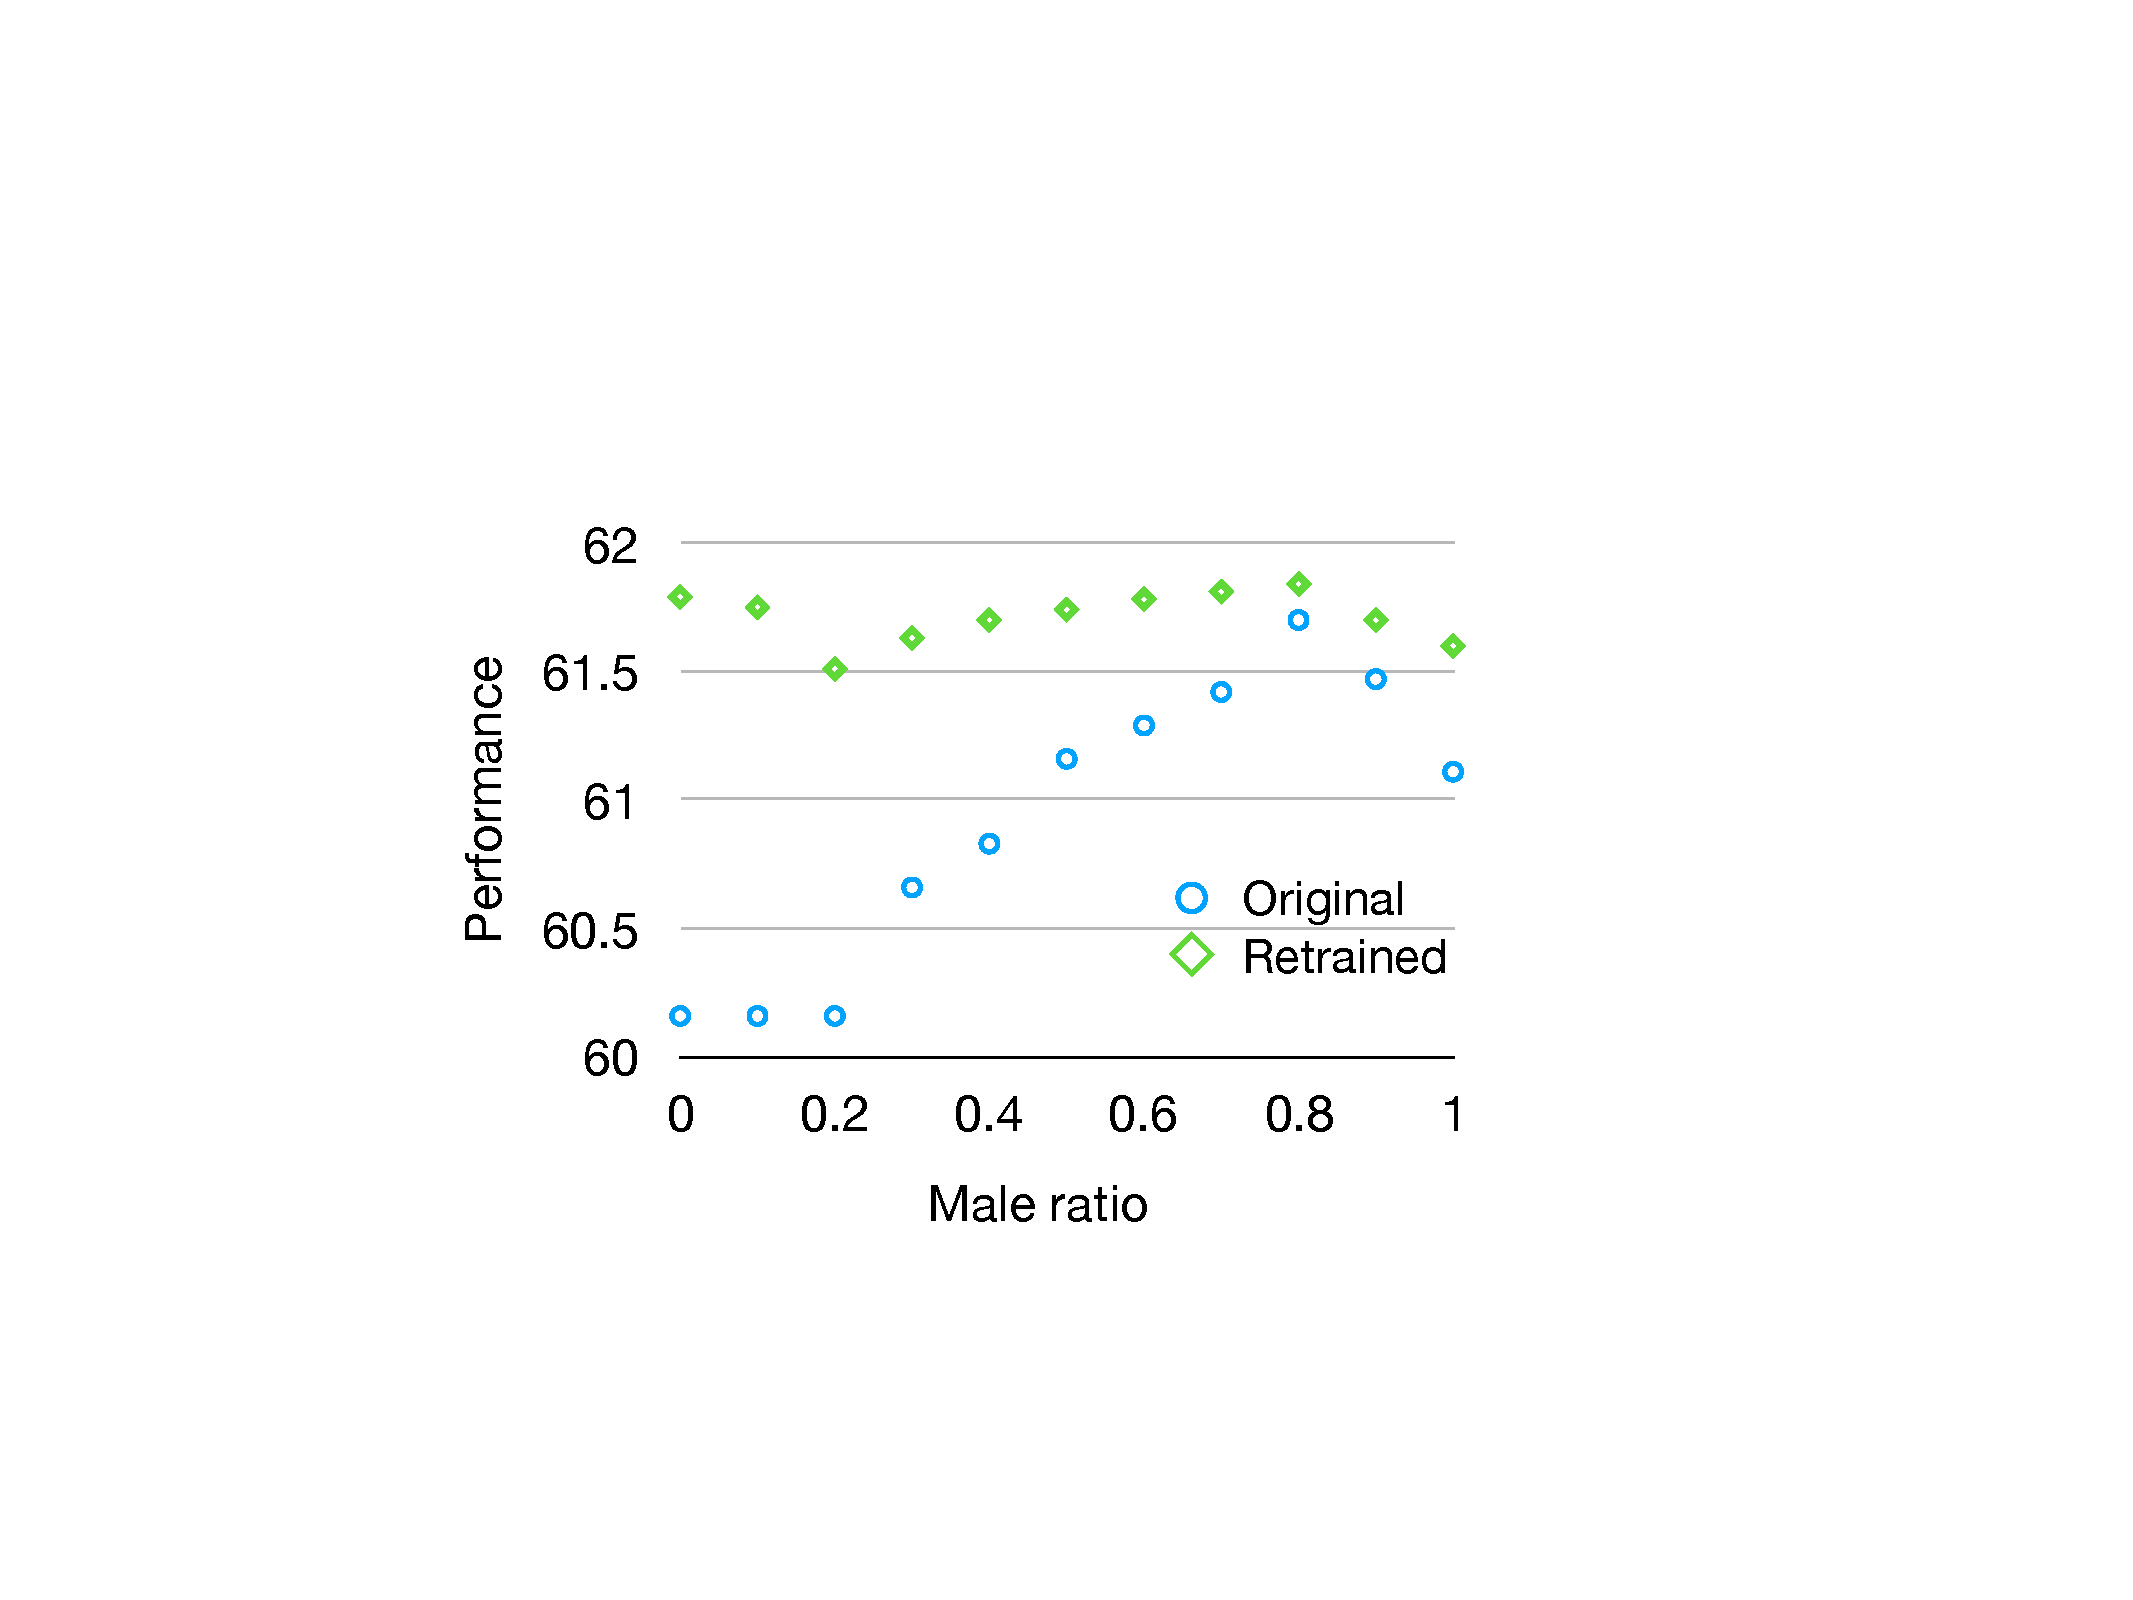
\includegraphics[width=1.0\linewidth]{figures/perf}
%         \caption{Performance with different male ratio distributions. Here the x-axis refers to the male gender ratio in the dataset and the y-axis is the model performance.}
%         \label{fig:performance}
% \end{figure}